% IF YOU CAN SEE THIS GO CONTRIBUTE >:(

\documentclass[letterpaper, 8pt]{extarticle}
\usepackage{amssymb,amsmath,amsthm,amsfonts}
\usepackage{multicol,multirow}
\usepackage{calc}
\usepackage{ifthen}
\usepackage[landscape]{geometry}
\usepackage[colorlinks=true,citecolor=blue,linkcolor=blue]{hyperref}

\usepackage{booktabs}
\usepackage{ulem}
\usepackage{enumitem}
\usepackage{tabulary}
\usepackage{graphicx}
\usepackage{siunitx}
\usepackage{tikz}
\usepackage{derivative}
\usepackage{svg}
\usepackage{listings}
\usepackage{setspace}
\usepackage{listings}
\usepackage{xcolor}
\usepackage{courier}
\usepackage{syntax}
\usepackage{mathpartir}
\usepackage{wrapfig}

% minimal line spacing
% \setstretch{0.1}

% set borders (experimentally determined to minimize cutoff and maximize space on school printers)
\geometry{top=.25in,left=.25in,right=.25in,bottom=.35in}

% make figures work better in multicol
\newenvironment{Figure}
{\par\medskip\noindent\minipage}
{\endminipage\par\medskip}

\pagestyle{empty} % clear page

% rewrite section commands to be smaller
\makeatletter
\renewcommand{\section}{\@startsection{section}{1}{0mm}%
                                {-1explus -.5ex minus -.2ex}%
                                {0.5ex plus .2ex}%x
                                {\normalfont\normalsize\bfseries}}
\renewcommand{\subsection}{\@startsection{subsection}{2}{0mm}%
                                {-1explus -.5ex minus -.2ex}%
                                {0.5ex plus .2ex}%
                                {\normalfont\small\bfseries}}
\renewcommand{\subsubsection}{\@startsection{subsubsection}{3}{0mm}%
                                {-1ex plus -.5ex minus -.2ex}%
                                {1ex plus .2ex}%
                                {\normalfont\tiny\bfseries}}
\makeatother
\setcounter{secnumdepth}{0} % disable section numbering


% disable indenting
\setlength{\parindent}{0pt}
\setlength{\parskip}{0pt plus 0.5ex}

% Custom siunitx defs
\DeclareSIUnit\noop{\relax}
\NewDocumentCommand\prefixvalue{m}{%
\qty[prefix-mode=extract-exponent,print-unity-mantissa=false]{1}{#1\noop}
}

% Shorthand definitions
\newcommand{\To}{\Rightarrow}
\newcommand{\ttt}{\texttt}
\newcommand{\ra}{\rightarrow}

% condense itemize & enumerate
\let\olditemize=\itemize \let\endolditemize=\enditemize \renewenvironment{itemize}{\olditemize \itemsep0em}{\endolditemize}
\let\oldenumerate=\enumerate \let\endoldenumerate=\endenumerate \renewenvironment{enumerate}{\oldenumerate \itemsep0em}{\endoldenumerate}
\setlist[itemize]{noitemsep, topsep=0pt, leftmargin=*}
\setlist[enumerate]{noitemsep, topsep=0pt, leftmargin=*}

\title{3GC3}

\begin{document}
\raggedright
\tiny

% make listings look nicer
\lstset{
	tabsize = 2, %% set tab space width
	showstringspaces = false, %% prevent space marking in strings, string is defined as the text that is generally printed directly to the console
	basicstyle = \tiny\ttfamily, %% set listing font and size
	breaklines = true, %% enable line breaking
	numberstyle = \tiny,
	postbreak = \mbox{\textcolor{red}{\(\hookrightarrow\)}\space}
}

\begin{center}
	{\textbf{2Z03 Exam}} \\
\end{center}
% set column spacing rules
\setlength{\premulticols}{1pt}
\setlength{\postmulticols}{1pt}
\setlength{\multicolsep}{1pt}
\setlength{\columnsep}{2pt}
\begin{multicols*}{4}

	\section{Trigonometry}
	\begin{align*}
		\csc \theta            & = 1/\sin\theta                                                \\
		\sec \theta            & = 1/\cos\theta                                                \\
		\sin(\pi/2 - \theta)   & = \cos \theta                                                 \\
		\cos(\pi/2 - \theta)   & = \sin \theta                                                 \\
		\cos(2 \theta)         & = \cos^2 \theta - \sin^2 \theta                               \\
		\cos(2\theta)          & = 2 \cos^2 \theta - 1                                         \\
		\cos(2 \theta)         & = 1 - 2\sin^2 \theta                                          \\
		\tan(2 \theta)         & = \frac{2\tan\theta}{1 - \tan^2 \theta}                       \\
		\sin\theta + \sin \phi & = 2 \sin(\frac{\theta +\phi}{2}) \cos(\frac{\theta - \phi}2)  \\
		\sin\theta - \sin \phi & = 2 \cos(\frac{\theta +\phi}{2}) \sin(\frac{\theta - \phi}2)  \\
		\cos\theta + \cos \phi & = 2 \cos(\frac{\theta +\phi}{2}) \cos(\frac{\theta - \phi}2)  \\
		\cos\theta - \cos \phi & = -2 \sin(\frac{\theta+ \phi}{2}) \sin(\frac{\theta - \phi}2) \\
		\sin\theta \sin\phi    & = \frac{\cos(\theta - \phi) - \cos(\theta + \phi)}{2}         \\
		\cos\theta \cos\phi    & = \frac{\cos(\theta - \phi) + \cos(\theta + \phi)}{2}         \\
		\sin\theta \cos\phi    & = \frac{\sin(\theta + \phi) + \sin(\theta - \phi)}{2}         \\
		\cos\theta \sin\phi    & = \frac{\sin(\theta + \phi) - \sin(\theta - \phi)}{2}         \\
		\sinh x                & = \frac{e^x - e^{-x}} 2                                       \\
		\cosh x                & = \frac{e^x + e^{-x}} 2                                       \\
	\end{align*}

	\section{Models}
	\textbf{Newton's Law of Cooling}
	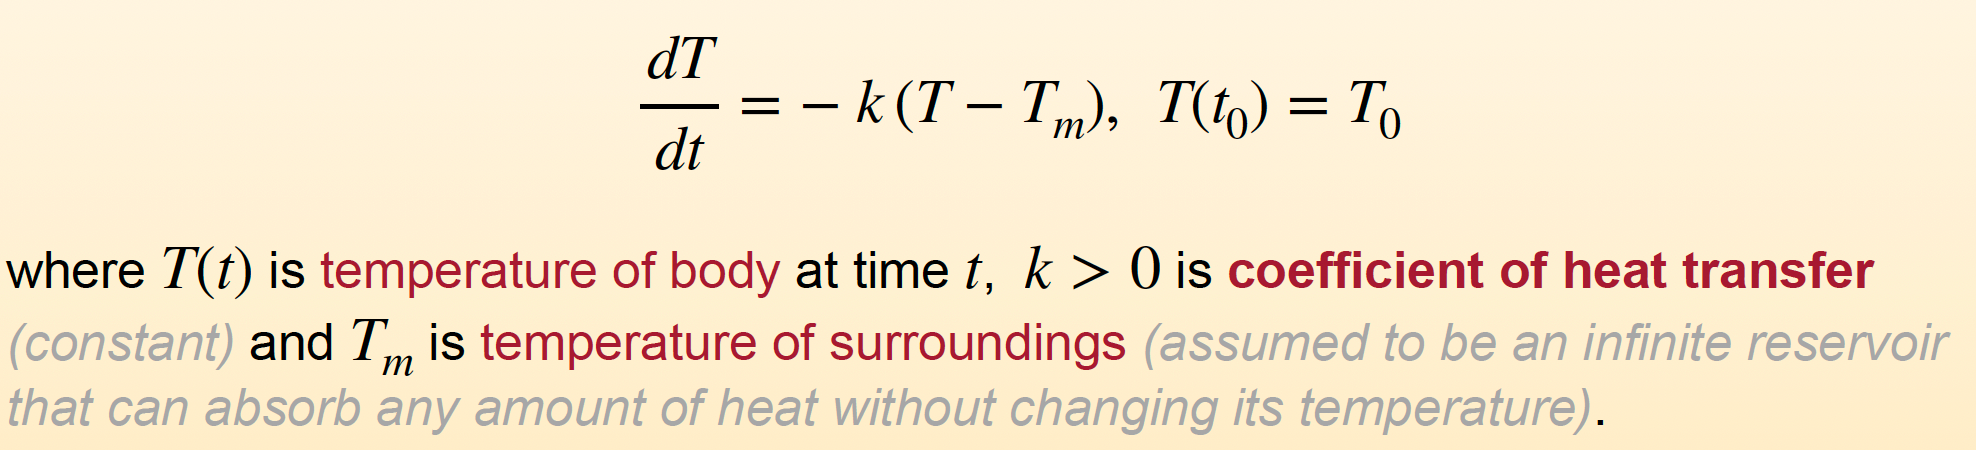
\includegraphics[width=\linewidth]{newtons-law-of-cooling.png}
	\begin{align*}
		T(t) & = T_m + (T_0 - T_m)e^{-k(t-t_0)}
	\end{align*}

	\textbf{Draining a Tank}
	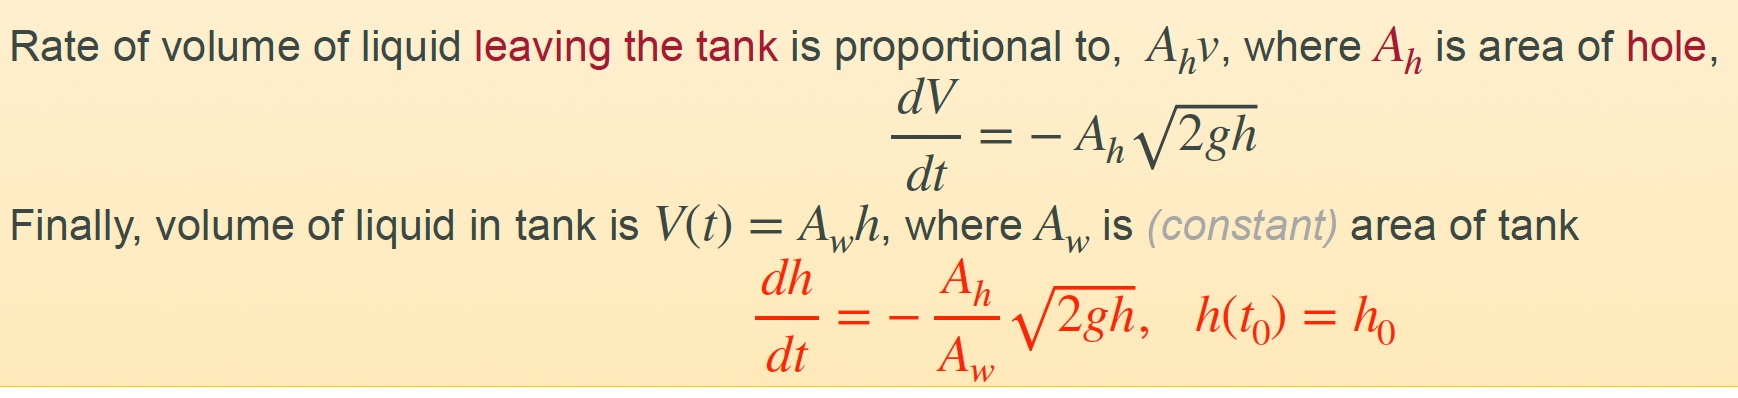
\includegraphics[width=\linewidth]{draining-a-tank.jpeg}
	\begin{align*}
		h(t) & = \left(h_0^{1/2} - \frac{A_h\sqrt{2g}}{2A_w}(t-t_0)\right)^2
	\end{align*}

	\textbf{Population Growth}
	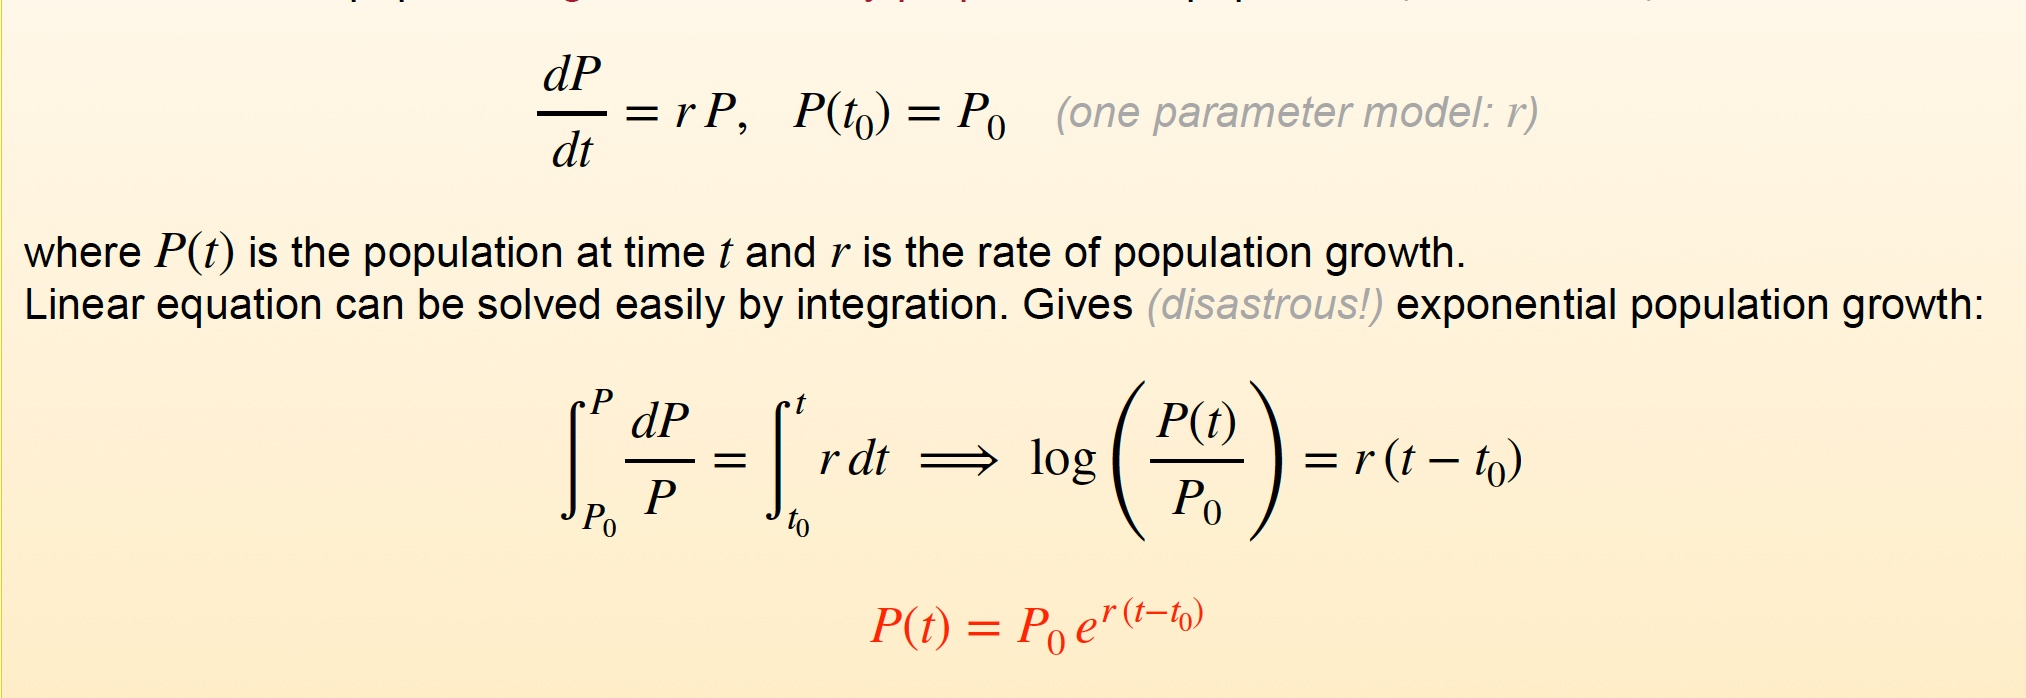
\includegraphics[width=\linewidth]{population-growth.jpeg}

	\textbf{Realistic Population Growth}
	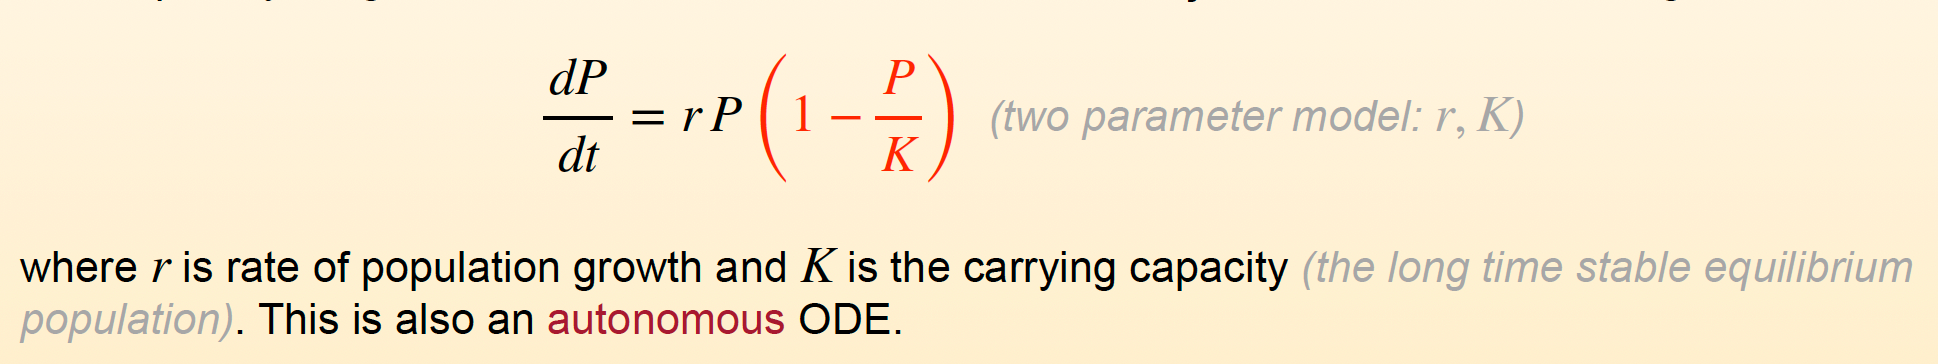
\includegraphics[width=\linewidth]{realistic-population-growth.png}
	\begin{align*}
		P(t) & = P_0\frac{K}{P_0 + (K - P_0)e^{-rt}}
	\end{align*}

	\textbf{Beem deflection} \\
	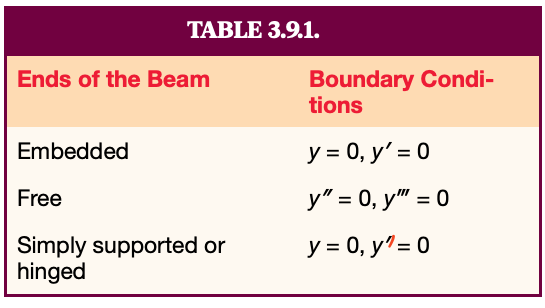
\includegraphics[width=0.6\linewidth]{beam-deflection.png} \\

	\textbf{Hook's Law of Springs} \\
	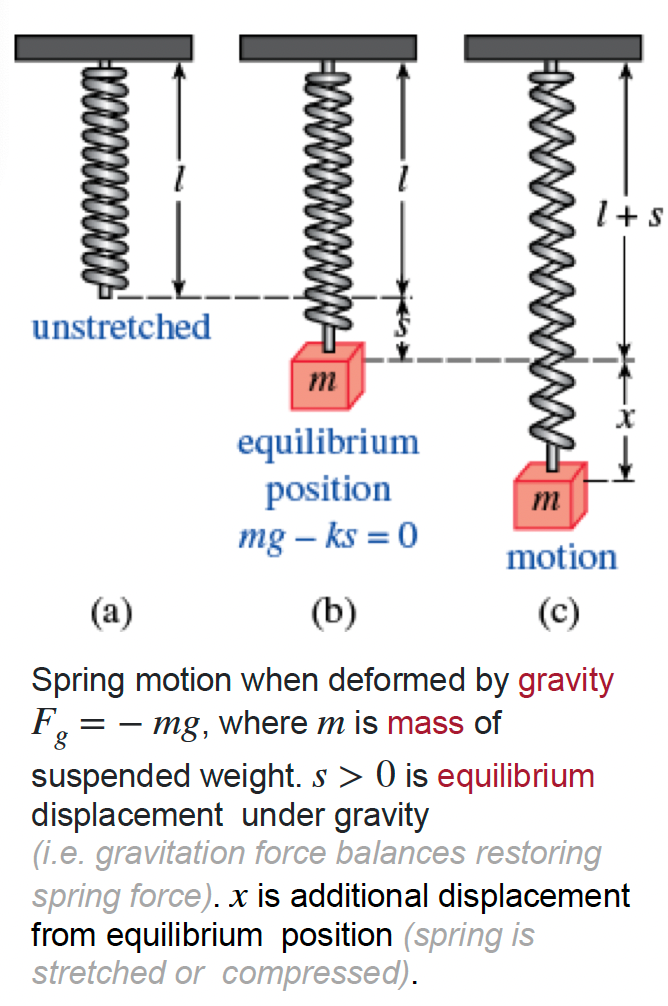
\includegraphics[width=0.6\linewidth]{hookes-law.png} \\
	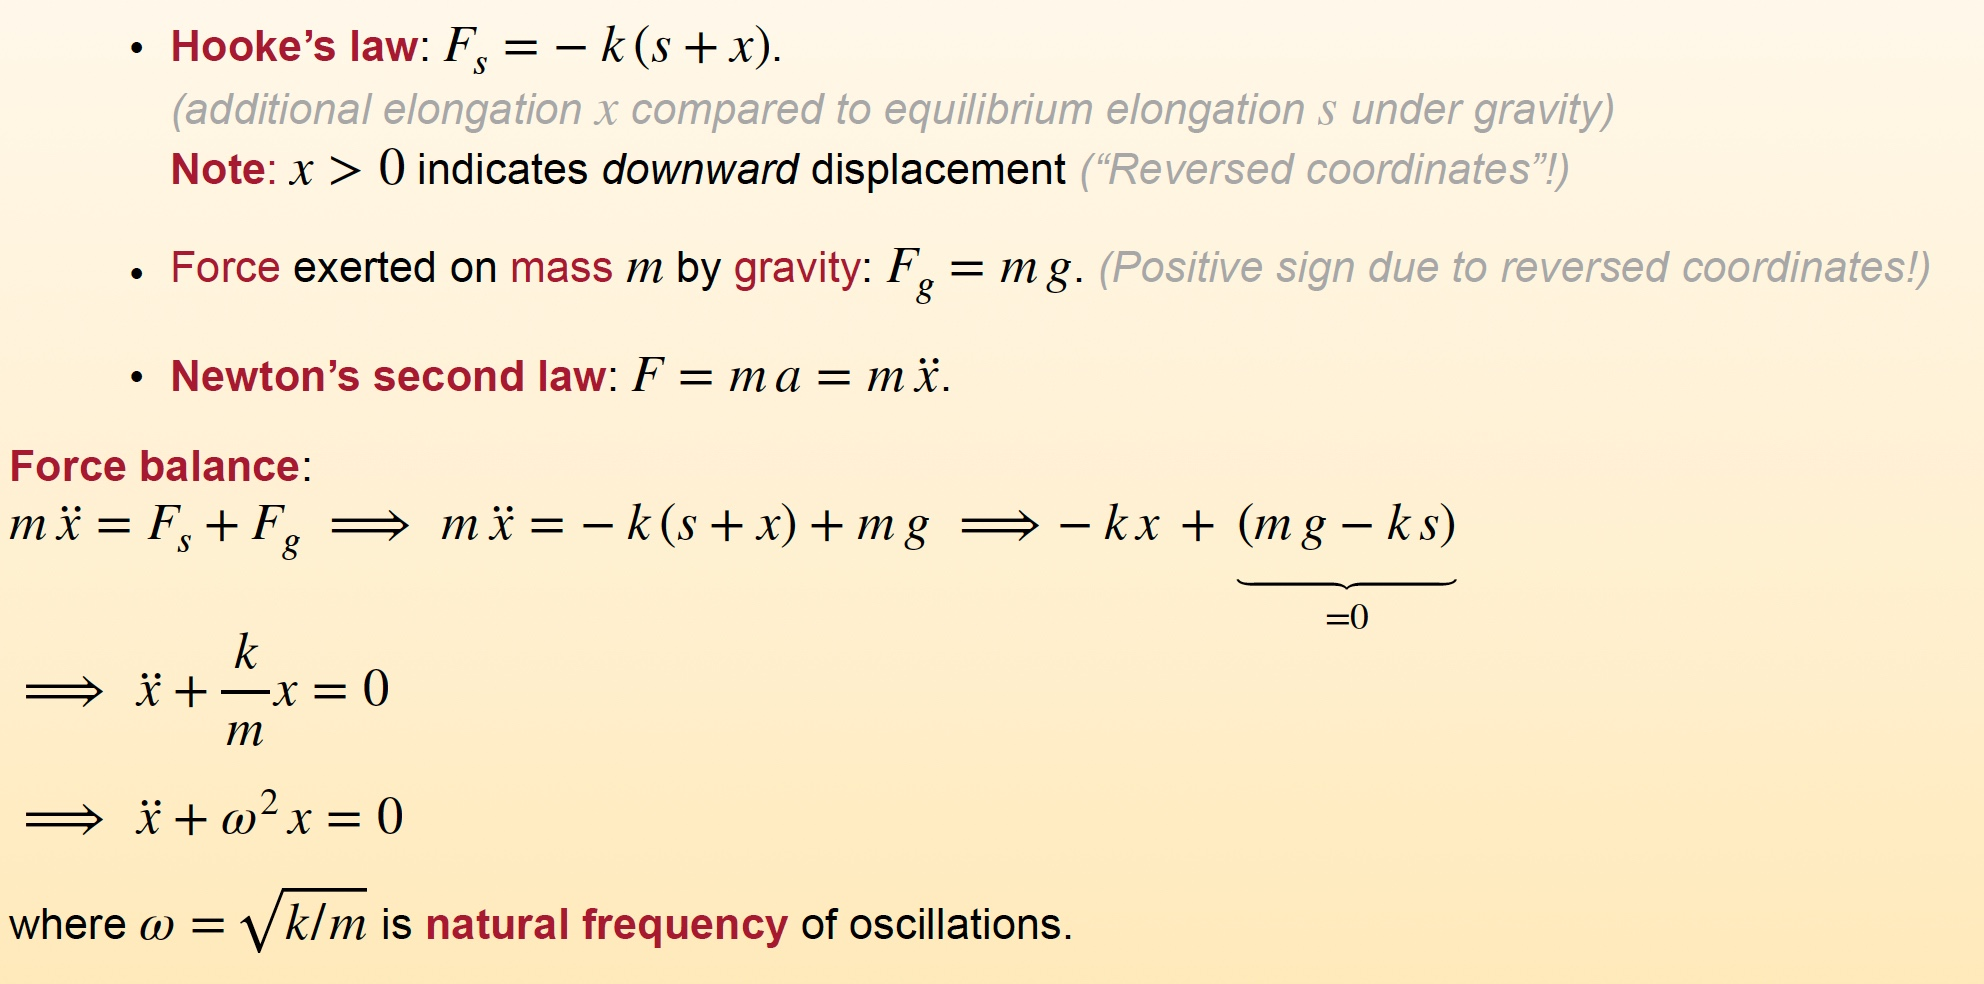
\includegraphics[width=\linewidth]{force-balancing.jpeg} \\
	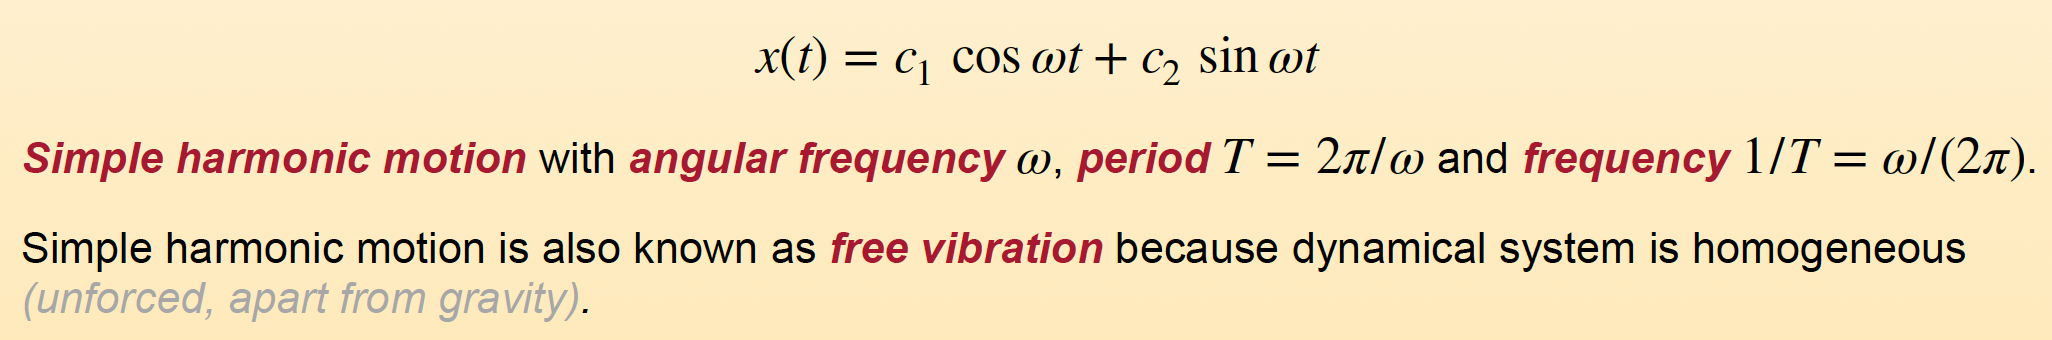
\includegraphics[width=\linewidth]{dynamic-system-spring-mass-forced-by-gravity.png} \\
	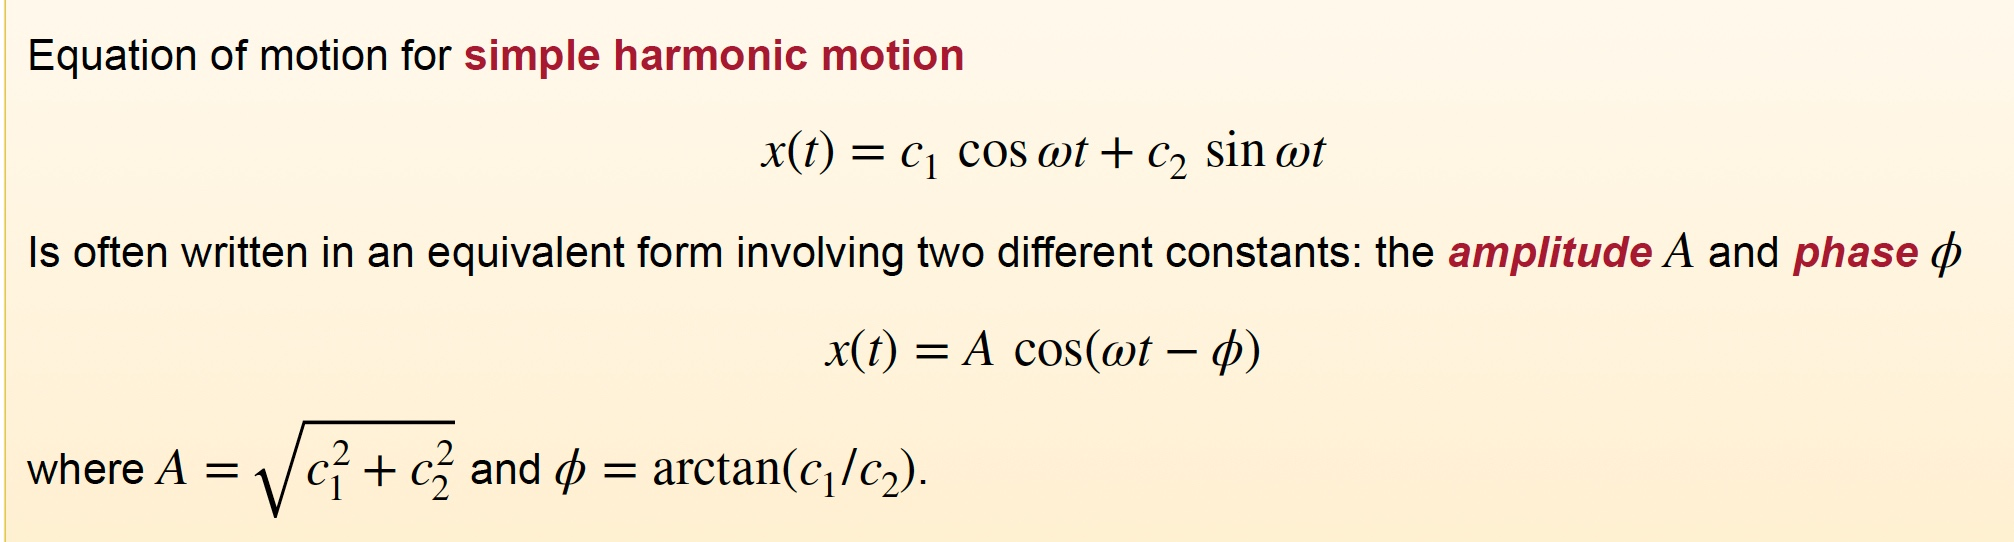
\includegraphics[width=\linewidth]{simple-harmonic-motion.jpeg} \\

	\textbf{Dampened spring system} \\
	\begin{align*}
		mx'' = -kx - \beta x'
	\end{align*}
	where $\beta > 0$ is \textbf{damping constant}.
	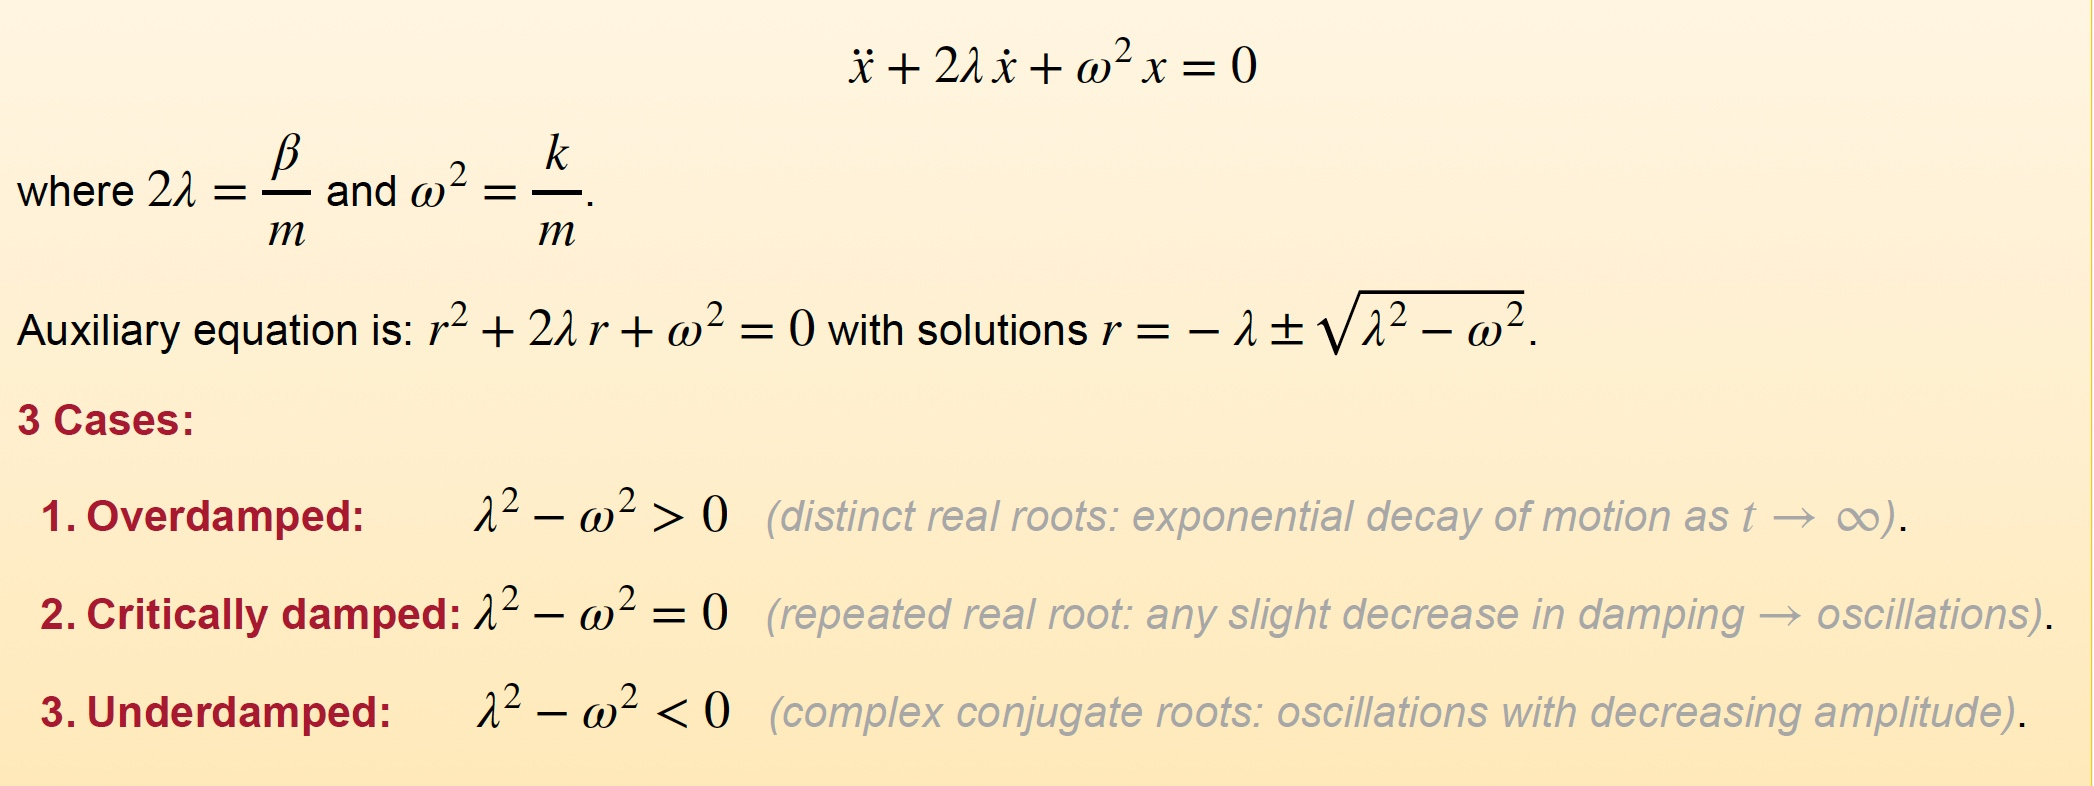
\includegraphics[width=\linewidth]{damped-system.jpeg} \\

	Can also apply external forcing:
	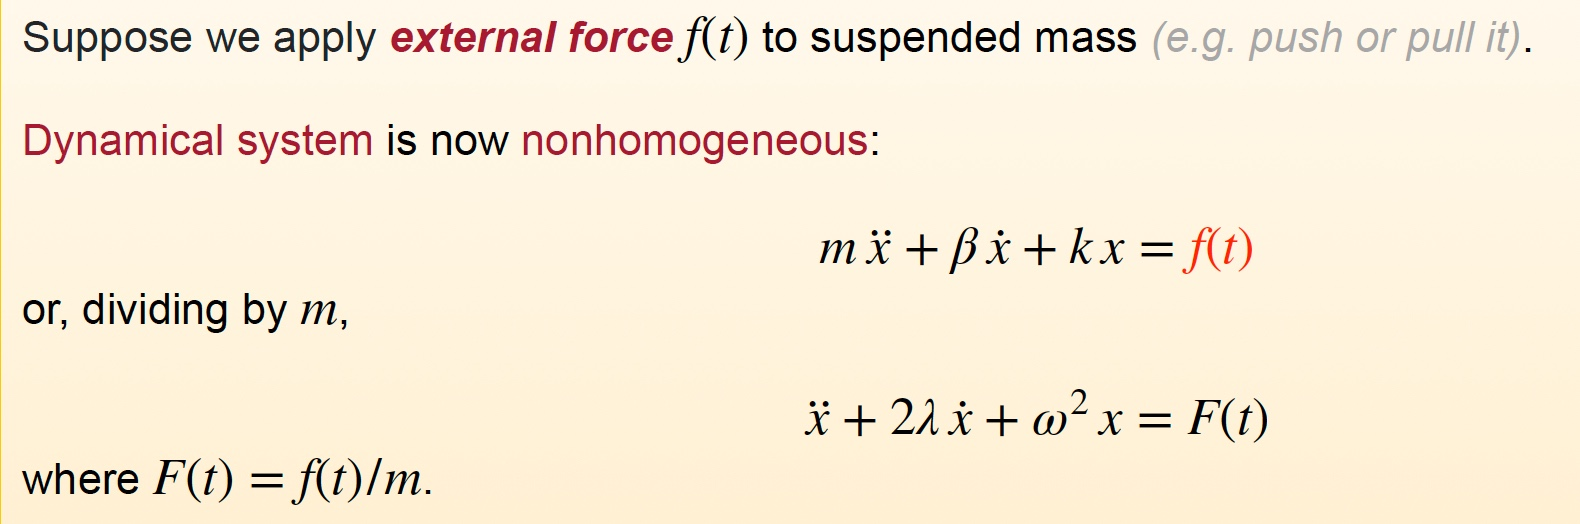
\includegraphics[width=\linewidth]{external-force.jpeg} \\

	\section{$L[y] = y'' + P(x)y' + Q(x)y = f(x)$}
	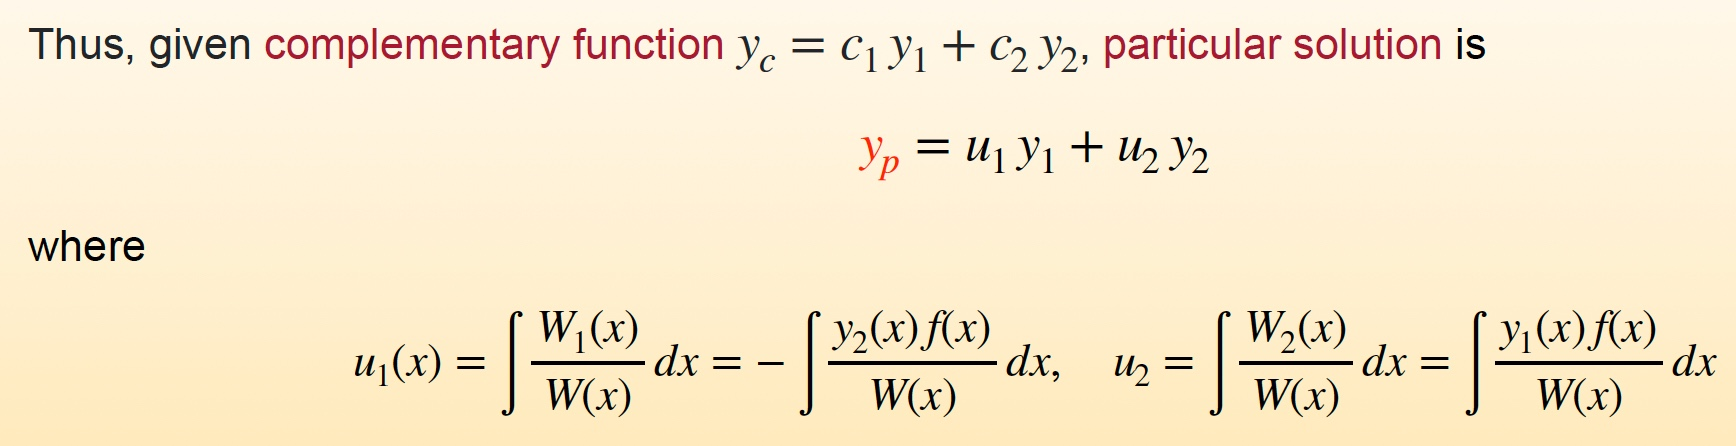
\includegraphics[width=\linewidth]{variation-of-parameters.jpeg} \\

	\section{Cauchy Euler Equations}
	General soloution is $y = x^{m}$:
	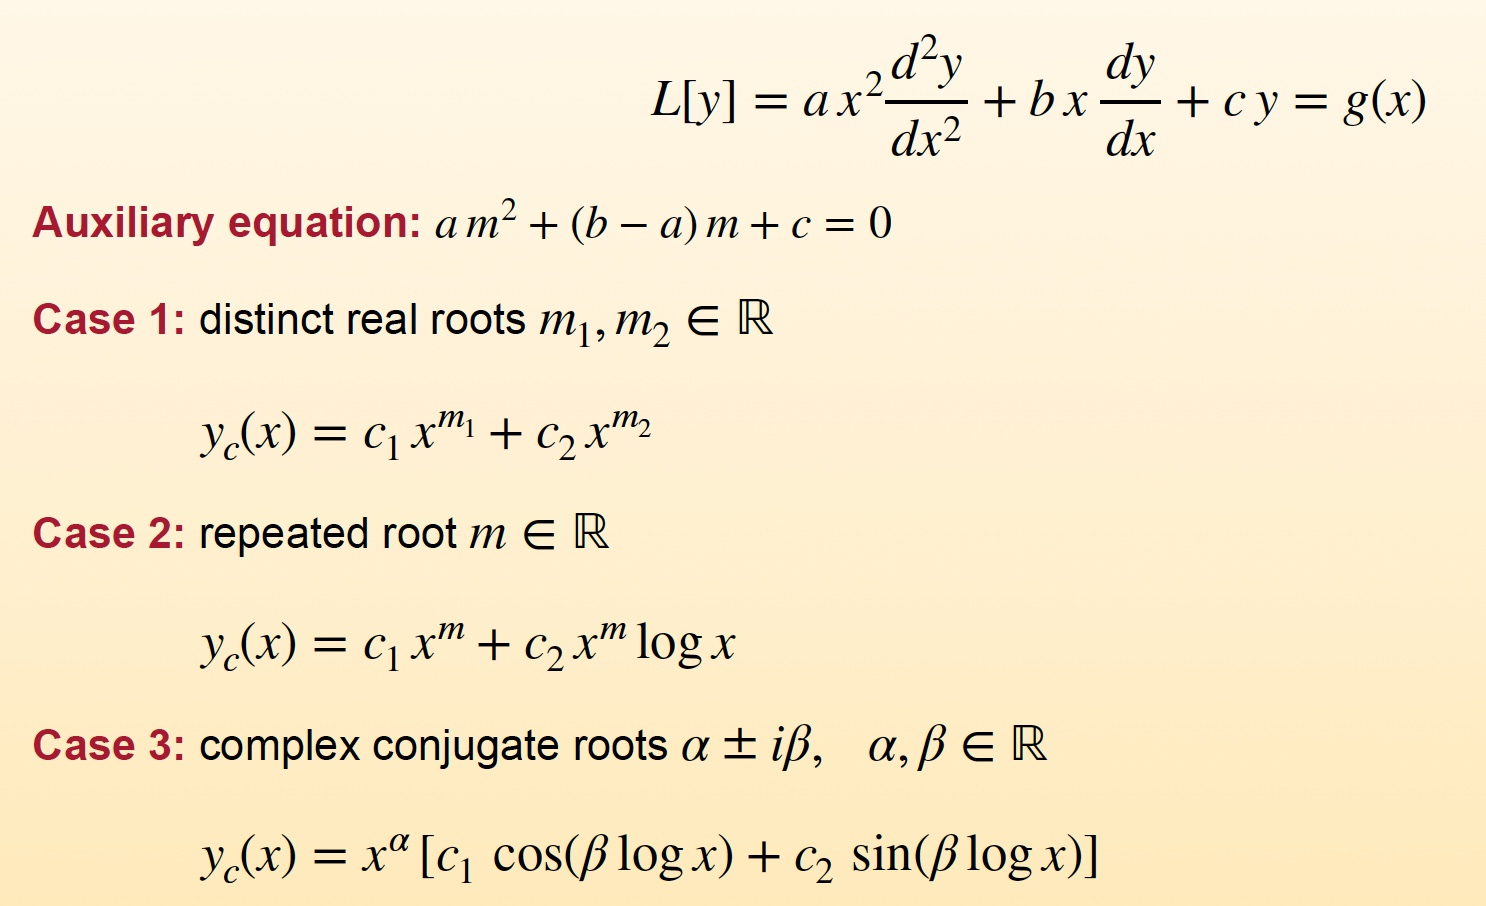
\includegraphics[width=\linewidth]{cauchy-euler-equations.jpeg} \\

	\section{Partial differential equations}
	\textbf{variations}
	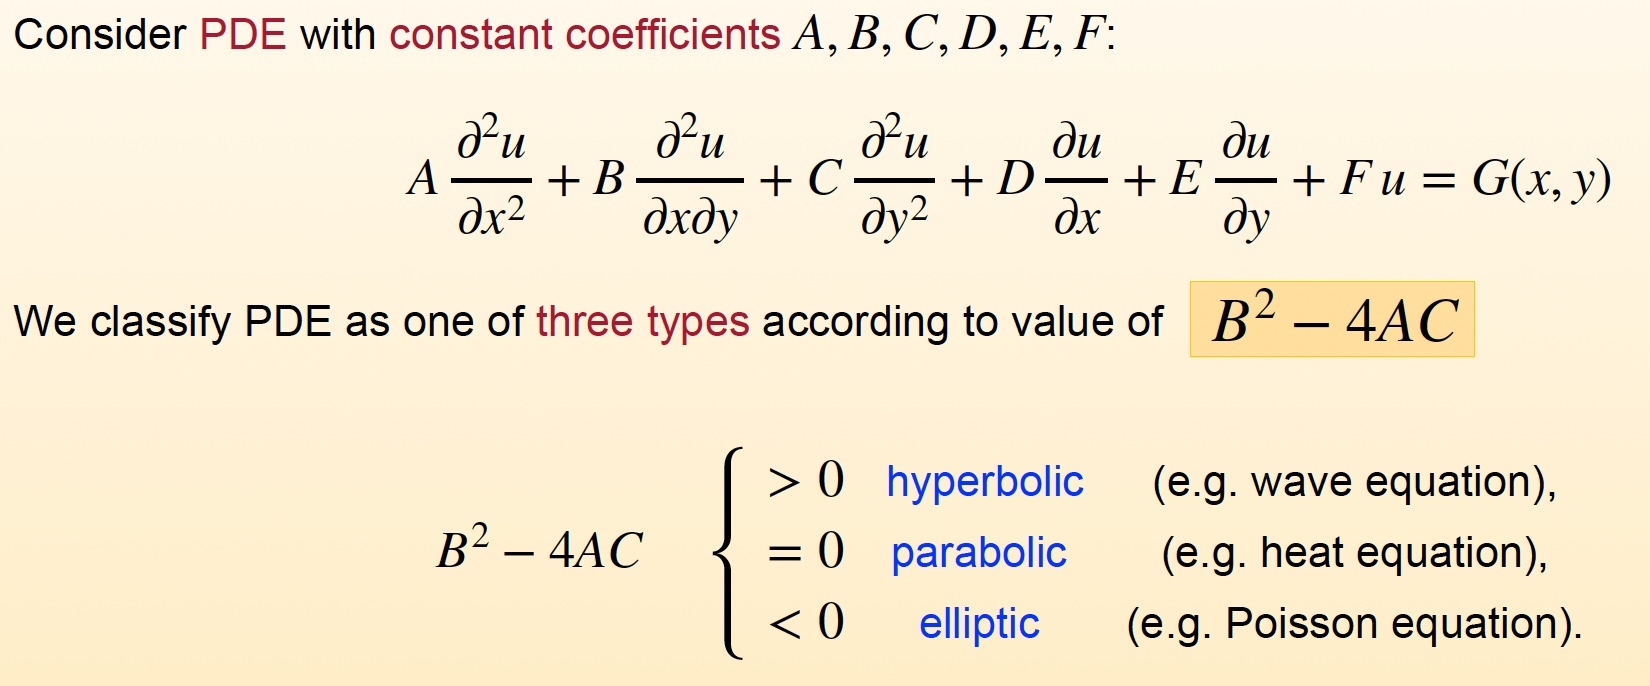
\includegraphics[width=\linewidth]{general-partial-eq.jpeg} \\
	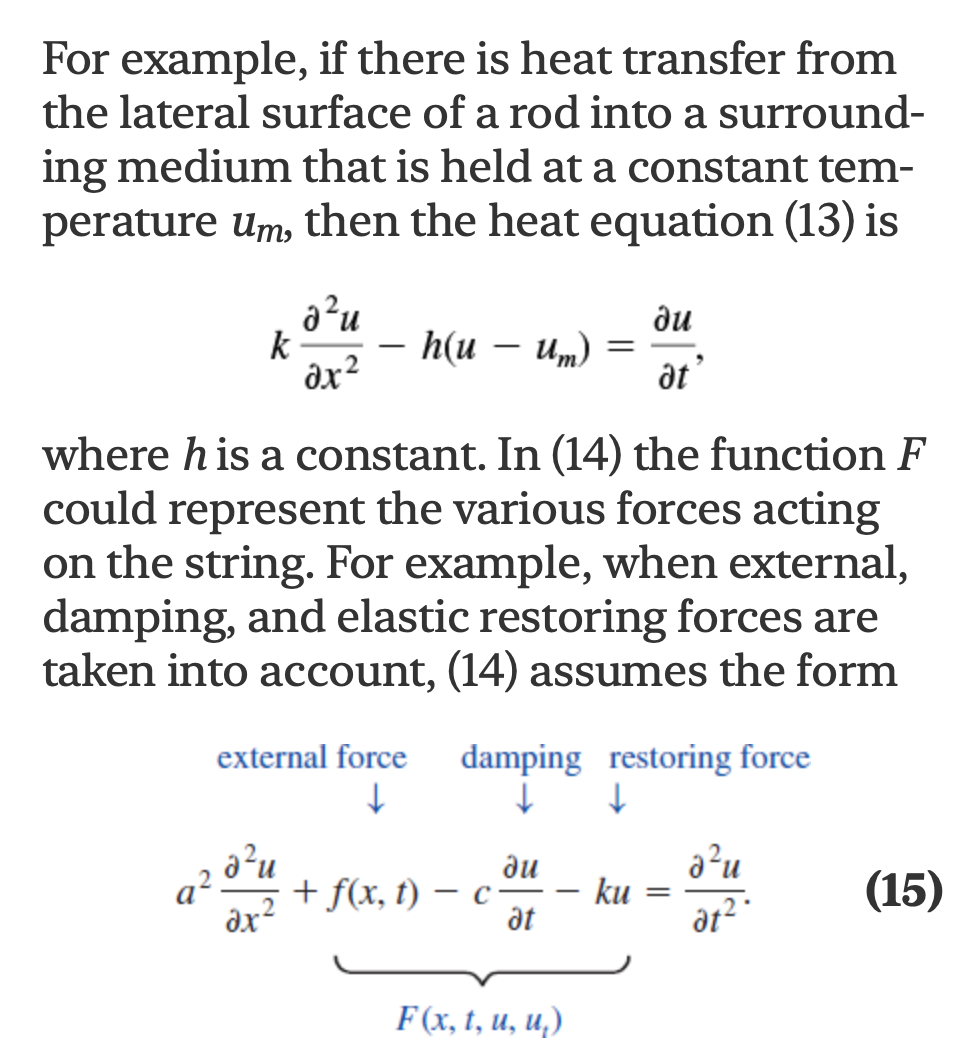
\includegraphics[width=\linewidth]{parital-eq-variations.png} \\

	\textbf{heat equation}
	\begin{align*}
		k \frac{\partial^2 u}{\partial x^2} & = \frac{\partial u}{\partial t}
	\end{align*}

	\textbf{wave equation}
	\begin{align*}
		a^2 \frac{\partial^2u}{\partial x^2} & = \frac{\partial^2 u}{\partial t^2}
	\end{align*}

	\textbf{laplace equation}
	\begin{align*}
		\frac{\partial^2u}{\partial x^2} + \frac{\partial^2 u}{\partial y^2} & = \rho(x, y)
	\end{align*}
	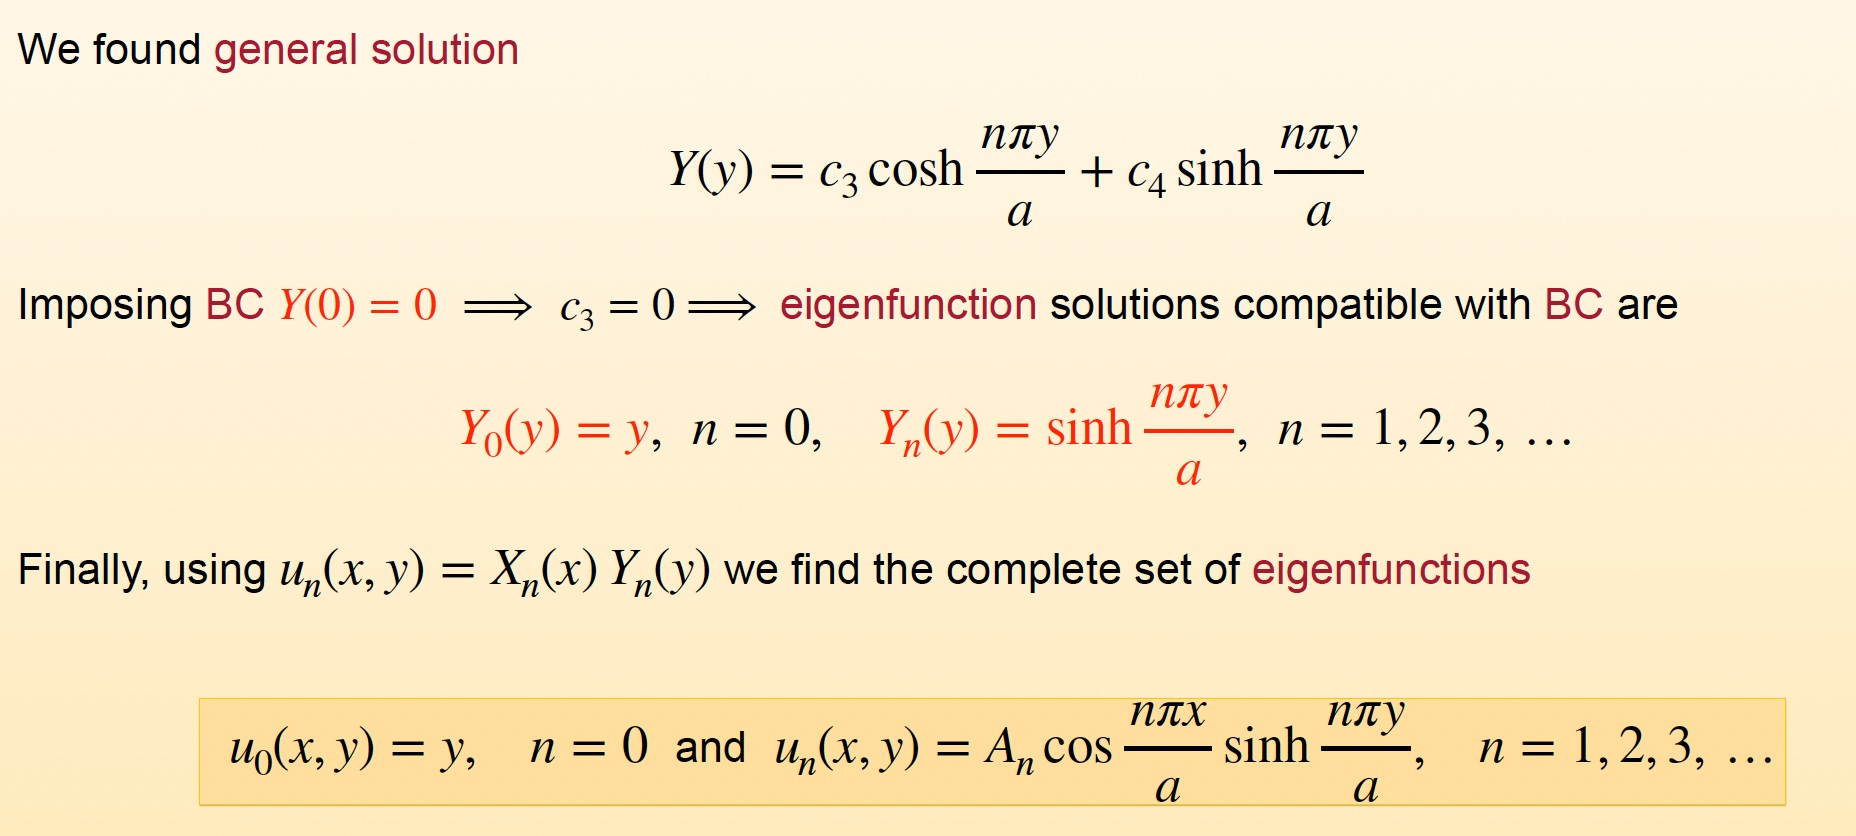
\includegraphics[width=\linewidth]{laplace1.jpeg} \\
	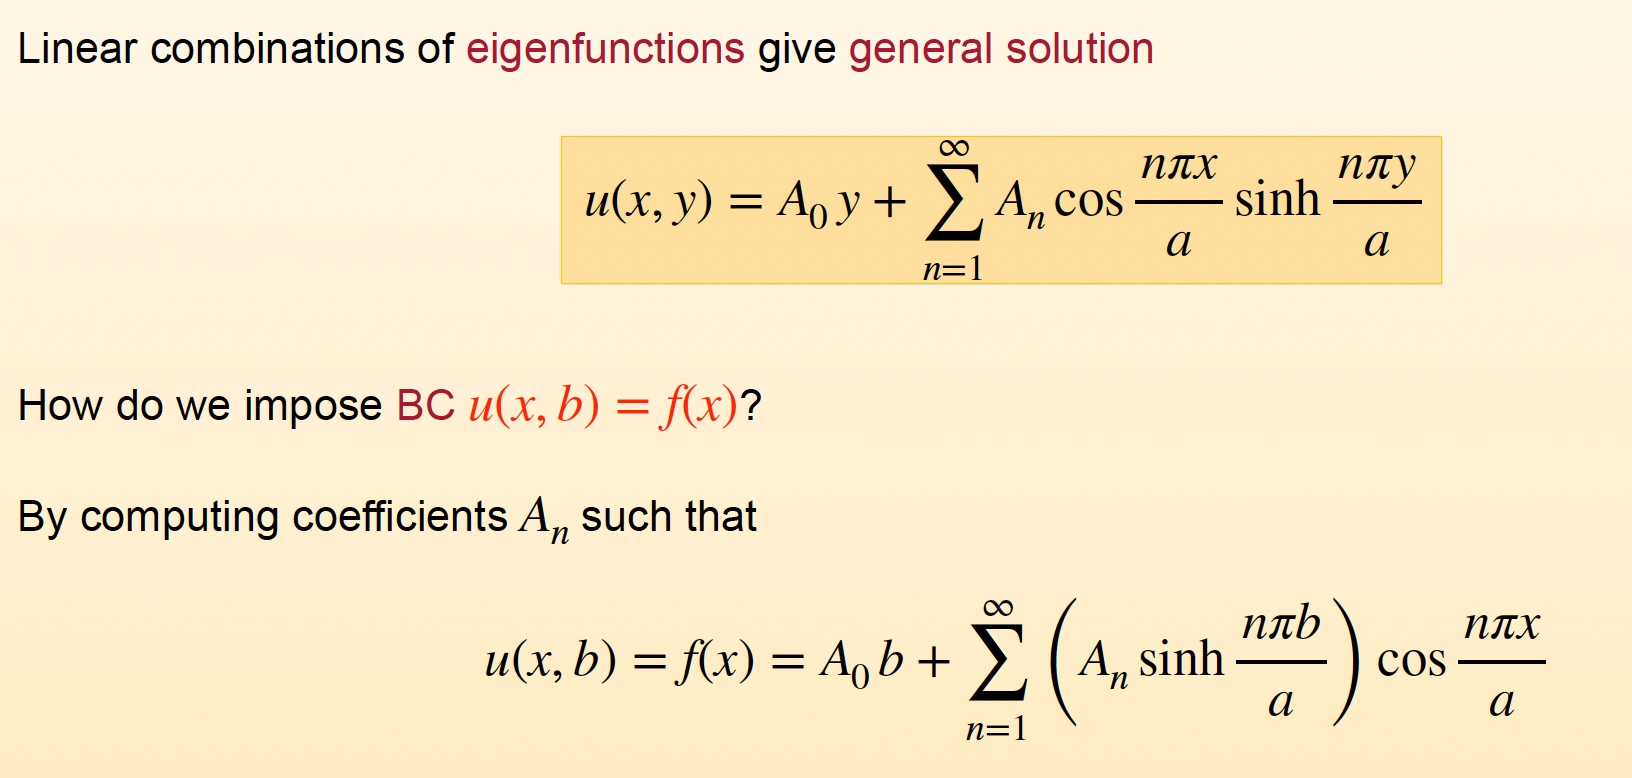
\includegraphics[width=\linewidth]{laplace2.jpeg} \\
	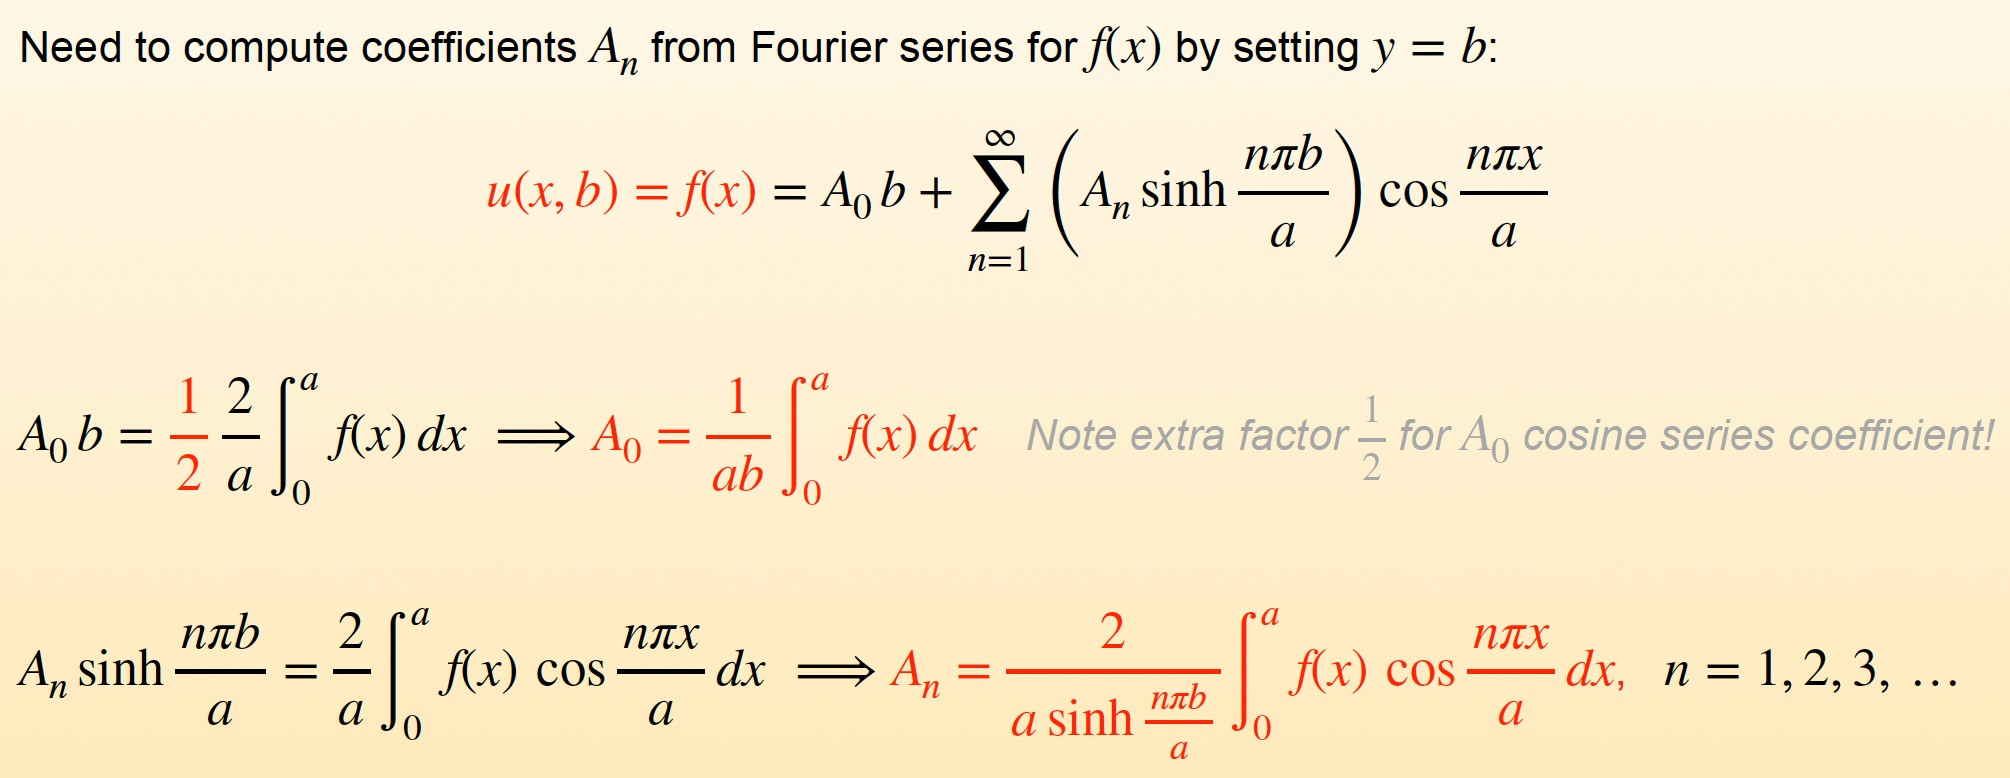
\includegraphics[width=\linewidth]{laplace3.jpeg} \\
	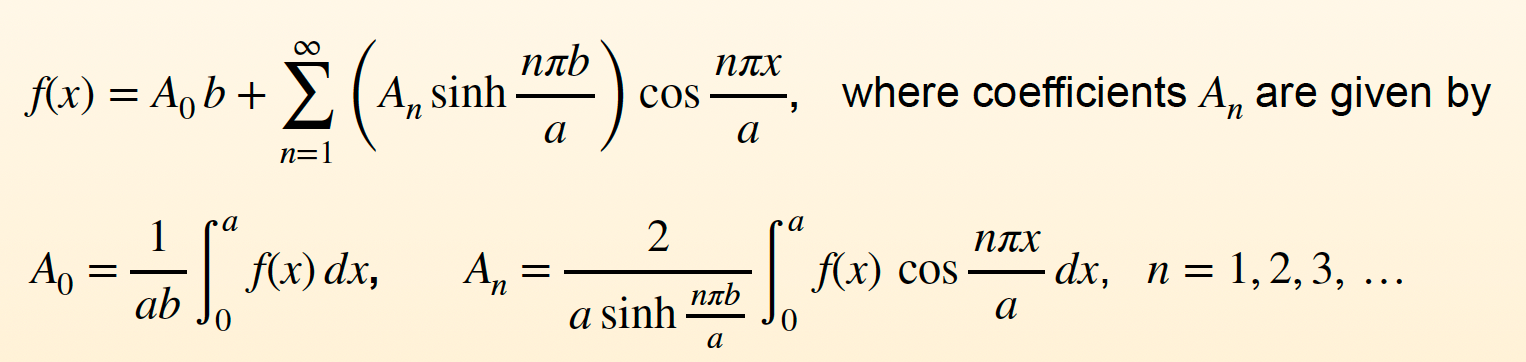
\includegraphics[width=\linewidth]{laplace4.png} \\

\end{multicols*}

\end{document}
